\subsection{Различение сигналов.}


В эксперименте формируется реализация $x(t)$, представляющая собой
аддитивную смесь шума $\xi(t)$ и одного из перечисленных ниже сигналов $m(t)$,
$x(t)=m(t)+ \xi(t)$. Сигнал выбирается по случайному равновероятному закону.
Требуется определить, какой из сигналов содержится в данной реализации при
отношении сигнал/шум 0.1.

\begin{table}[H]
    \centering
    \small
    \begin{tabular}{|c|c|c|c|c|}
    \hline
    Вид сигнала & Амплитуда & \makecell{Длитель- \\ность, мс} & \makecell{Средняя частота \\
    заполнения, Гц} &
    \makecell{Девиация \\                        частоты, Гц} \\
    \hline 
    \makecell{ ЛЧМ импульс с \\ нарастающей частотой} & $\sqrt 2$& 100 & 2000 & 300 \\
    \hline 
\makecell{ ЛЧМ импульс с \\ убывающей частотой} & $\sqrt 2$& 100 & 2000 & 300 \\
    \hline 
\makecell{Код Баркера (N=13) \\ с гармоническим заполнением } & $\sqrt 2$& 100 & 2000 & 300 \\
    \hline 
    \makecell {Код Баркера (N=13)  \\ зеркально
отражённый  \\
относительно \\ 
вертикальной оси\\ с гармоническим заполнением} & $\sqrt 2$& 100 & 2000 & 300 \\
    \hline
    \end{tabular}
\end{table}


Когда мы будем сравнивать перечисленные сигналы, то даже при малом ОСШ
можно однозначно идентифицировать необходимый сигнал, если фильтр настроен на
него. Если фильтр согласован с сигналом, то этот сигнал будет отличаться от
остальных  меньшей длительностью и большей
амплитудой (см.рис. \ref{fig:6.1} - \ref{fig:6.4}). 



\begin{figure}[H]
    \centering
    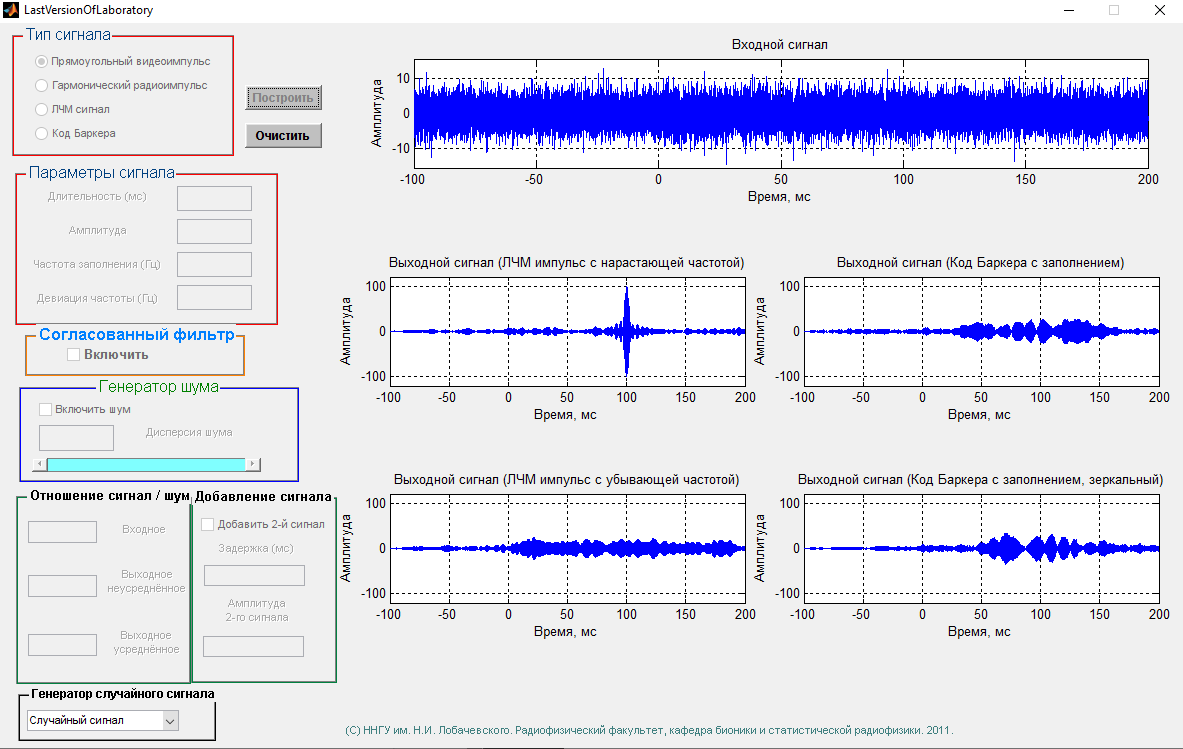
\includegraphics[width=\linewidth]{imgs/task6/lfm}
    \caption{}
    \label{fig:6.1}
\end{figure}

\begin{figure}[H]
    \centering
    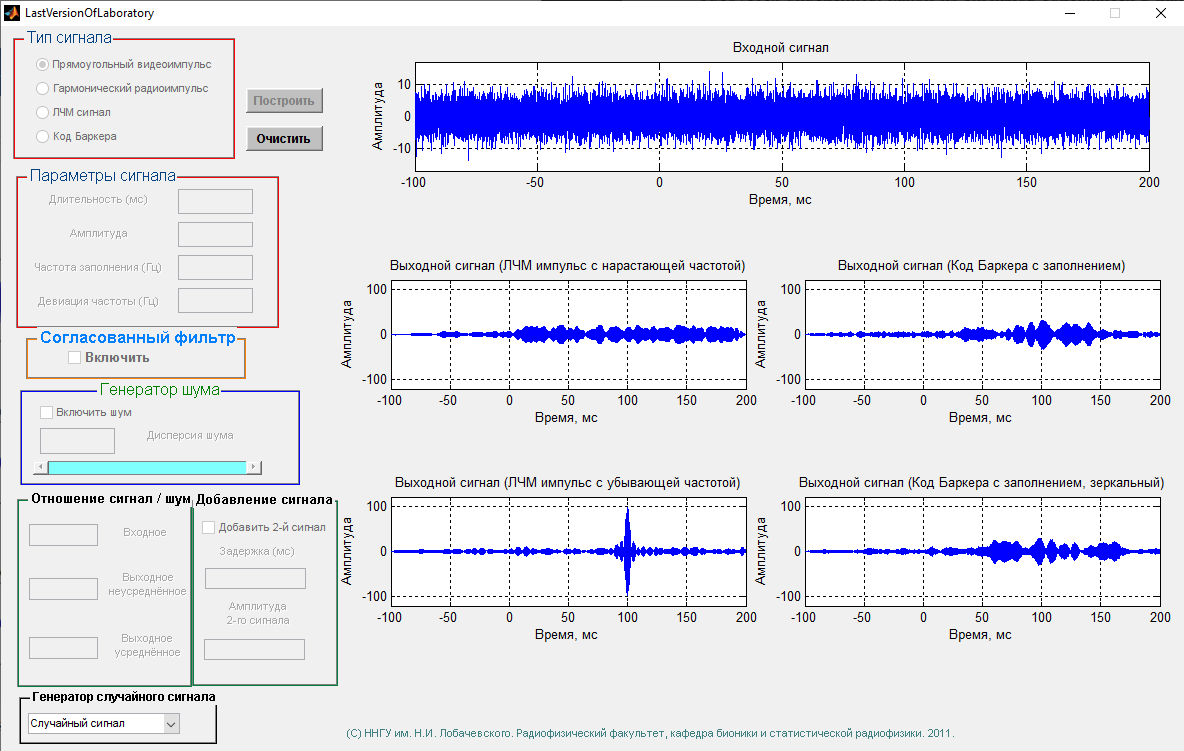
\includegraphics[width=\linewidth]{imgs/task6/lfm_mirror}
    \caption{}
    \label{fig:6.2}
\end{figure}

\begin{figure}[H]
    \centering
    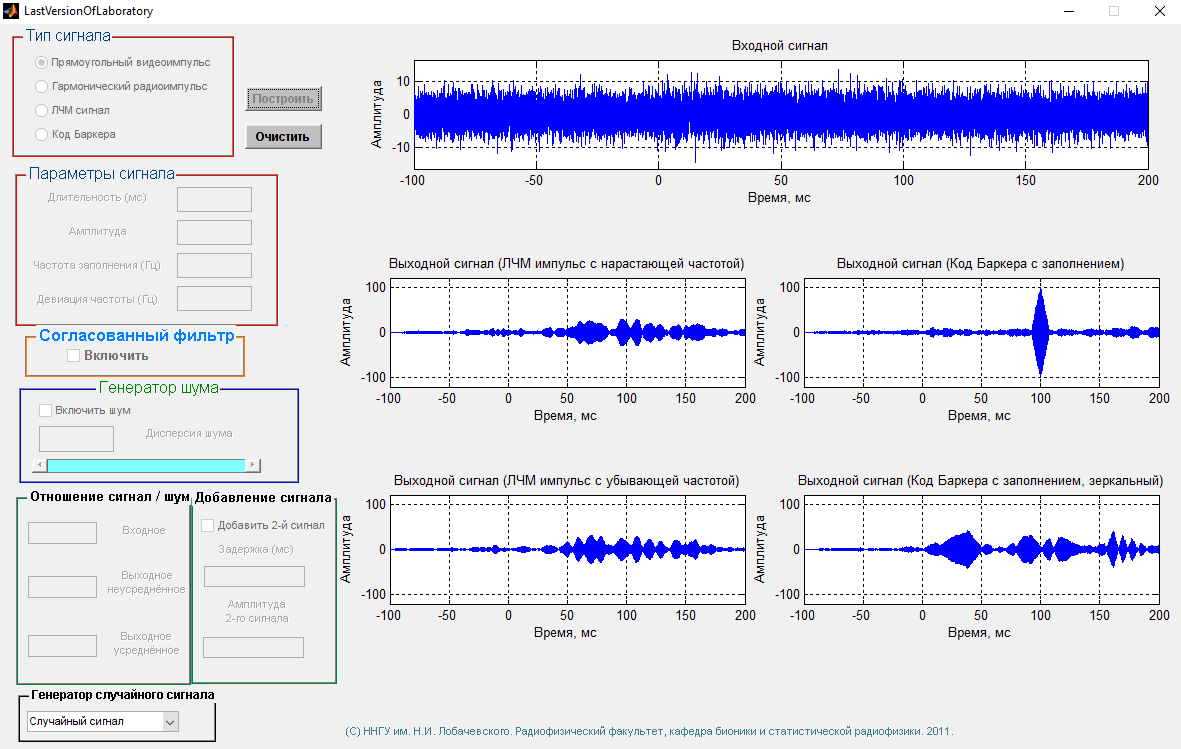
\includegraphics[width=\linewidth]{imgs/task6/barker}
    \caption{}
    \label{fig:6.3}
\end{figure}

\begin{figure}[H]
    \centering
    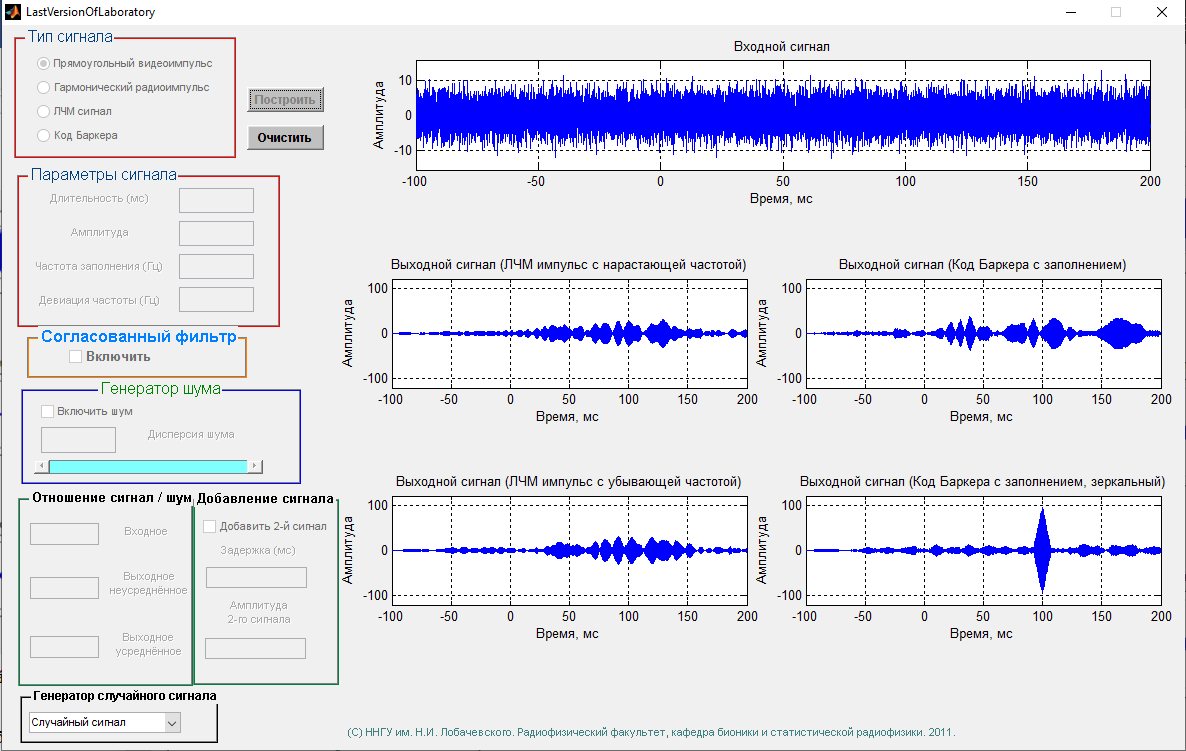
\includegraphics[width=\linewidth]{imgs/task6/barker_mirror}
    \caption{}
    \label{fig:6.4}
\end{figure}
